\documentclass[a4paper,11pt]{book}
\usepackage[utf8]{inputenc}
%% Packages for maths.
\usepackage{amsmath}
\usepackage{amstext}
\usepackage{amsfonts}
%\usepackage{bm}
%\usepackage{nicefrac}
% Packages to make the document nicer.
%\usepackage{color}
\usepackage {fancyhdr}
\usepackage{fontspec}
\setmainfont[Mapping=tex-text]{Verdana}
\setmonofont{Courier New}
%%%%%%%%%%%%%%%%%%%%%%%%%%%%%%%%%%%%%%%%%
\usepackage[a4paper]{geometry}
	\geometry{verbose,tmargin=2cm,bmargin=2cm,lmargin=1.5cm,rmargin=1.5cm,headheight=1cm,headsep=1cm,footskip=1cm}
	\setcounter{secnumdepth}{4}
	\setcounter{tocdepth}{4}
	\setlength{\parindent}{1cm}
	\pagestyle{fancy}
	\lhead{}
	\chead{Documentation in progress. Sorry for unnoticed changes.}
	\rhead{}
	\lfoot{Universidad Complutense de Madrid}
	\cfoot{\thepage}
	\rfoot{}
	\renewcommand{\headrulewidth}{0.4pt}
	\renewcommand{\footrulewidth}{0.4pt}

%%%%%%%%%%%%%%%%%%%%%%%%%%%%%%%%%%%%%%%%%
%\usepackage{multirow}
%\usepackage{array}
% \usepackage{tablefootnote}
\usepackage{graphicx}
%\usepackage{wrapfig}
% \usepackage{caption}
%\usepackage{subcaption}
\usepackage[unicode=true,
bookmarks=true,bookmarksnumbered=false,bookmarksopen=false,
breaklinks=true,pdfborder={0 0 1},backref=false,colorlinks=false]
{hyperref}
\hypersetup{pdftitle={LELAPE},
	pdfauthor={Francisco J. Franco}}
%%%%%%%%%%%%%%%%%%%%%%%%%%%%%%
\usepackage{tcolorbox} 
%%% https://tex.stackexchange.com/questions/66154/how-to-construct-a-coloured-box-with-rounded-corners
%%%%%%%%%%%%%%%%%%%%%%%%%%%%%%%
\begin{document}

\title{
\includegraphics[width=10cm]{fig/LELAPE_LOGO.png}\\ \Huge{\textbf{LELAPE}}}
\author{\href{https://www.ucm.es/ghadir}{GHADIR Group} \\ \href{https://www.ucm.es}{Universidad Complutense de Madrid} \\ \vspace{1cm}\\  
\includegraphics[height=4.5cm]{fig/Ghadir_group.jpg}\hspace{1cm} 
\includegraphics[width=4cm]{fig/logo_ucm.png}}
\date{}



\frontmatter
\maketitle
\tableofcontents

\mainmatter
\chapter{Introduction}
%
\section{The reason of using LELAPE}
Probably, you are reading this document because you are a researcher that tests electronica devices under radiation. Even more, perhaps you are not interested in any electronic devices but, at this very moment, only in commercial-off-the-shelf (COTS) memories. 

Under the wide umbrella of memories, different devices are comprised. Let us enumerate some of them:
%
\begin{itemize}
	\item Static Random Access Memories (SRAMs)
	\item Dynamic Random Access Memories (DRAMs), but also Synchronous DRAM (SDRAMs) and Pseudo-Static RAMs (PSRAMs)
	\item Non-volatile memories (Flash, PRAM, MRAM, etc.)
	\item Configuration memory in FPGAs
	\item Cache memory in microprocessors and microcontrollers
	\item ...
\end{itemize}
%
It is well known that these elements will undergo bitflips after an exposition to protons, neutrons, heavy ions, ... The common test procedure is to write a pattern in the memory and look for errors in a later  read-back. These errors will be labeled indicating the word address and the flipped-bit position in the word. 

Unfortunately, this is the so-called \textit{physical address} and it is impossible to relate it to the exact physical position on the integrated circuit. And this leads to a serious problem at the time of interpreting results. Nearby bitflips are probably caused by pernicious multiple cell upsets (MCUs) but they will not discovered unless the researcher has somehow got the information to relate the logical address to its physical counterpart (an X, Y pair on the silicon surface).

However, the presence of MCUs will leave a signature in the set of the logical addresses of bitflips, which can be used to group pairs of related bitflips and classify them in single or multiple events. No matter are the multiple events hidden among the rest of bitflips, we can track and locate them.

\textbf{LELAPE} is the Spanish acronym for \textit{Listas de Eventos para Localizar Anomalías Preparando Estadísticas}, which is equivalent in English to LAELAPS (\textit{Lists of All Events for Locating Anomalies by Preparing Statistics}). In Greek mythology, LELAPE, or LAELAPS, is Zeus' hound, with the magic skill to track and hunt any prey however hidden it may be. In a similar way, LELAPE is a software tool able to inspect sets of apparently random logical addresses of bitflips and discover those that are members of the same multiple event.

LELAPE can be found on Zenodo (\href{https://zenodo.org/records/10156119}{https://zenodo.org/records/10156119}), with assigned DOI:  10.5281/zenodo.10156119, or in the GitHub website (\href{https://github.com/fjfrancopelaez/LELAPE}{https://github.com/fjfrancopelaez/ LELAPE}), where development releases are available.

\section{Acnowledgments}
%
This tool was supported by the Spanish ``\textit{Ministerio de Ciencia e Innovación (MICINN)}'' by means of the PID2020-112916GB-I00 project.
\section{How to reference LELAPE}
%
If you have successfully used this tool and the results are worth for academic publications, we ask you for including the following references:
%
\begin{itemize}
	\item Please, this site, or the ZENODO repository with DOI:10.5281/zenodo.10156119.
	\item \textbf{The Julia Language}: J. Bezanson, A. Edelman, S. Karpinski, and V. B. Shah, \textit{“Julia: A fresh approach to numerical computing},” SIAM review, vol. 59, no. 1, pp. 65–98, 2017 (DOI: 10.1137/141000671).
\end{itemize}
%
Last reference is independent of LELAPE but related to the Julia Language instead. Its authors ask for including this reference to follow the use of Julia in science.
%
\section{License of use}
%
LELAPE is released under the European Union Public Licence v. 1.2. Terms of use are at public display on \href{https://github.com/fjfrancopelaez/LELAPE/blob/main/LICENSE}{https://github.com/fjfrancopelaez/LELAPE/blob/main/LICENSE}. 



\chapter{Theoretical Background}
\section{Memory devices as a metric space-like sets}
First of all, we are going to depict a memory as a set of ordered elements, which can contain only two possible values. Clearly, this elements are the memory cells, and values are \textbf{0} \& 1.

As the set is ordered, we can assign an index number to every cell, which will be a positive natural number. For example, in FPGAs, this index is the position of the bit in the bitstream. In SRAMs, we can assign any cell the following index:
%
\begin{equation}
	Index = ADD\times W + k
	\label{Eq:PseudoAddressDefinition}
\end{equation}
%
\(ADD\) being the word address, \(W\) the wordwidth, and \(k\) the bit positiion in the word. From now on, we will call this index as \textit{pseudoaddress} in SRAMs. As this definition is arbitrary, anyone can postulate others for the \textit{pseudoaddress}, keeping in mind that any new definition  must be bijective. Thus, 
\[
	Index_2 = ADD\times W + (W-k)
\]
could also be valid.

It is immediate that the memory size, \(L_N\) is the number of available cells. If this memory is divided in \(L_A\) \(W\)-bit width words, \(L_N = L_A\times W\) holds.  In the simplest scenario, cell indexes are distributed between \(0\) and \(L_N-1\),  but more complicated situations can occur:
%
\begin{itemize}
	\item In some microcontrollers, we can download its content as a binary file and the SRAM memory is placed between \(A_0\) \& \(A_0+L_N-1\) positions. Other memories such as the Flash memory are in other parts of the file.
	\item In Xilinx FPGAs, the downloaded bitstream contains information about the configuration memory, flipflops, and BRAM. The content of these parts are split in several pieces and inserted in the bitstream. It is necessary to perform some reverse engineering studies to gather information about how to disassemble the bitstream. Therefore, there will be gaps in the indexes.
\end{itemize}
%
The first case is easy to solve just correcting the offset, although under some circumstances this is not strictly necessary for reasons to be explained later. In the second case, some ideas are remove gaps one by one, keep the indexes as they are, etc. It is not so obvious how to proceed. 

We are going to defina a \textit{pseudodistance} or \textit{pseudometric} as any funcition \(d:\mathbb{N} \times \mathbb{N} \rightarrow \mathbb{N}\) such that:
%
\begin{enumerate}
	\item \(d(a, a) = 0\quad\forall a \in \mathbb{N}\)
	\item \(d(a, b) = 0\Leftrightarrow a = b \quad\forall a, b \in \mathbb{N}\)
	\item \(d(a, b) = d(b, a) \quad\forall a, b \in \mathbb{N}\)
\end{enumerate}
%
In this list, the triangular property (\(d(a,c) \le d(a, b)+d(b,c) \quad\forall a, b, c \in \mathbb{N}\)) has not been included. If the function fulfills this fourth condition, it would become a true distance or metric.

We will focus on two functions, which have proven to provide interesting results to analyze events. These are:
%
\begin{itemize}
	\item \textbf{Bitwise XOR}: Addresses are expressed in binary format and the distance is the result of making XOR operation on pairs of bits in the same position.
	\item \textbf{Positive subtraction}:  Or \textit{absolute subtraction}. It is defined as \(d(a, b)=\left|a-b\right|\). This function is a true metric.
\end{itemize}
%
Now, we can briefly return to the case of memory blocks in microprocessors, exposed in previous paragraphs. In spite of the fact that the addresses values could range from \(A_0\) to \(A_0+L_N-1\), values of the positive subtraction are restricted to \(0,\cdots, L_N-1\), and the same occurs for bitwise XOR is, e. g., \(A_0\) is a power of 2 higher than \(L_N\).
%
\section{Characteristics of subsets with randomly picked elements}
%
Let us come back to the simplest case: cell indexes are distributed between \(0\) \& \(L_N-1\). Let us suppose that we randomly pick \(N_{BF}\) cells, and we can choose a cell twice or more times. This is exactly what happens when a memory is irradiated: cells are randomly flipped (at least if multiple events do not occur) so, when the memory is read back, the addresses of flipped cells should be randomly distributed. Let us call this set of addresses \(ADD\)

In this case, it is possible to demonstrate several properties. For example, assuming that a cell can be hit twice, hence undetected, the expected actual number of flipped cells is:
\begin{equation}
	N_{BF}^* = N_{BF}+\frac{N_{BF}^2}{L_N}
	\label{Eq:ActualNumberOfBF}
\end{equation}
This correction is not necessary for typical experiments \footnote{Nevertheless, we have found it necessary for Monte-Carlo tests} so we will assume hereafter that the number of observed bitflips (\(N_{BF}\)) is just the total number, \(N_{BF}^*\). 

Now, we will build a new set, which we will call \textit{'``Difference Vector (DV)''}, as the pseudodistance values of all possible pairs of addresses of flipped cells:
%
\begin{equation}
	DV = \left[x = d(a, b) \quad \forall a, b \in ADD, b>a\right]
	\label{Eq:DefinitionOfDV}
\end{equation}
%
Some properties of this set are:
%
\begin{itemize}
	\item In \(DV\), there are \begin{equation}N_{DV}=\frac{1}{2}\cdot N_{BF}\cdot \left(N_{BF}-1\right) \label{Eq:SizeOfDV}\end{equation} elements, but this is valid only for results with one writing \& reading cycle. If there were several rounds, as it occurs in pseudostatic or dynamic tests, \(N_{DV}\) should be computed as the sum of the sizes of the partial sets.
	\item No element is \(0\). The reason is that every address appears once and only once.
	\item Some values can randomly appear several times in the \(DV\) set.
\end{itemize}
%
This last statement is extremely interesting. It is possible to deduce that, if only single bit upsets occur and the bitwise XOR is used \cite{Franco2017}, the expected number of values appearing \(k\) times in the \(DV\) set is:
\[
	N_{R,XOR}\left(k, N_{DV}\right) = \left( \begin{matrix} N_{DV}\\ k \end{matrix} \right) \cdot \frac{\left(L_N -1\right)^{N_{DV}-k}}{L_N^{N_{DV}-1}}
\]
In the case of using the positive subtraction \cite{Fabero2020}, the expression is more complicated but computable:
\[
	N_{R,POS}\left(k, N_{DV}\right) =\left( \begin{matrix} N_{DV}\\ k \end{matrix} \right) \cdot \sum_{i=0}^{N_{DV}-k}{\frac{(-1)^i}{i+k+1} \cdot \left( \begin{matrix} N_{DV}-k\\ k \end{matrix} \right) \cdot \frac{2^{i+k}}{L_N^{i+k-1}}}
\]
Whichever expression we choose, the expected number of repetitions fades away as \(k\) grows. Thus, it is possible to calculate the value of \(k_{th}\) from which the number of expected elements repeated \(k > k_{th}\) times is lower than \(\varepsilon\), with \(1\gg \varepsilon > 0\). Therefore, it is almost impossible to find elements in the \(DV\) set repeated more the \(k_{th}\) times. 

But this is true only if there are SBUs. If besides SBUs there are multiple cell upsets (MCUs), it is possible to find elements in the \(DV\) set repeated a forbidden number of times. These values are the marks of multiple events, that can be used to reconstruct the number and size of multiple events.

For example, in Example 5 of Jupyter notebooks, we discovered that there was overabundance of 1, 2, 3230--3234 in the \(DV\) set derived from results in an FPGA with positive subtraction. Pairs of flipped bit addresses differing in one of these values are very likely members of a single multiple event. A later study showed that the FPGA configuration memory is organized in columns of 101 32-bit words, hence the physical meaning of 3232 = 32 $\times$ 101, so cells differing 3232 are just in the same row.
%
\section{Methods to find and reject anomalously repeated value}
%
\subsection{The Self-Consistency Rule}
Experiments on actual devices show that some values appear in the \(DV\) set far more than expected. However, not all of them are marks to relate adjacent cells. 

Let us put an example. We have a hypothetical memory where cells are distributed along a simple chain, as in the bitstream of FPGAs. Now, let us suppose that 1 is a true mark to detect events, and that there are 2-bit MCUs in positions (100, 101), (350, 351), and (1500, 1501). As there are 6 cells, we can calculate 15 distances, the values of which appear the following number of times:
%
\begin{itemize}
	\item 1 : 3 times
	\item 150, 1150, 1400: 2 times
	\item 149, 151, 1149, 1151, 1399, 1401: once
\end{itemize}
%
As expected, 1, the true mark, appears more times than the rest of elements. However, three nonsense numbers, 150, 1150 and 1400, appear also several times since they measure the relative distance between identical-shape groups.

This phenomenon is exacerbated if larger events are present. In order to discard false events, we have proposed to include the ``\textit{self-consistency rule}''. The group of confirmed anomalous values are picked one by one from the set of anomalies following the number of occurrences. When the size of the predicted events is larger than the number of collected critical elements, the process takes a step back to discard the recently added elements and exits. The advantage of this rule is that nonsense anomalies are rejected, with the penalty of possibly discarding genuine anomalies. However, previous experiences led us to consider that this decision is better than to be too permissive and to accept false values, that eventually lead to the detection of unrealistic very large events, fruit of the artificial union of two or more unrelated small ones.
%
\subsection{The MCU rule}
%
Let us suppose that we have performed the self-consistency test on a set of addresses of flipped cells and that we have discovered several anomalies that allowed us reconstructing the possible multiple events. 

Let us focus now on those events with a size of 3 or more. Cells in every event are obviously adjacent, and perhaps, studying the relation between pairs cells inside every MCU we can discover new critical anomalies that were not discovered during the first check.

In LELAPE, only those anomalies found in MCUs that also appear more than expected are included in the list of genuine marks of events.
%
\subsection{The Trace rule}
% 
We call ``\textit{trace}'' of a natural number as the number of ones present in the binary expression of the number. When the bitwise XOR operation is used, discovered anomalies are usually values with only one to three values in binary format. 

Therefore, the rule is simple: let us check all the possible natural numbers lower than the memory size with low values of trace (1--3) to verify if they appear too often in the \(DV\) set. If so, they will be added to the group of confirmed anomailes. 

However, our experience shows that only values with traces of 1 or 2 are good candidates. Trace 3 is risky and 4 or higher are forbidden in LELAPE.
%
\subsection{The Shuffle rule}
%
The idea is quite simple. Let us suppose that, after applying previous rules we have discovered a set of anomalies. The idea behind this rule is to combine them in pairs using the distance function in order to obtain new values, and adding them to the set of anomalies if they appear in the \(DV\) set more than predicted by the statistical model.
%
\subsection{The History rule}
%
This is not exactly a rule, but a sign of being sensible. Let us suppose that you test a device and get a set of anomalies, \(A_1\). Later, you test it again and the obtained values are \(A_2\). As the device is the same, or at least of the same model and the anomalies are linked to the internal structure, it is evident that elements in \(A_1\) are valid for the second experiment, and vice versa. Thus, the union of both sets, \(A_1 \cup A_2\) can be used to classify results from both experiments.

Even more, if you had previously tested the device and identified a significant set of anomalies, it is possible to skip the process of obtaining anomalies and straightly apply that set on the test results, saving analysis time.
%
\section{Number of false events}
%
Sometimes, two or more single bit upsets may occur in adjacent cells in such a way that a later analysis can erroneously conclude that both belong to a unique multiple cell upset \cite{Tausch2009}. This is completely false, and the number of expected false events increases with the number of bitflips. It is possible to deduce that that number increases with the number of flipped bits, and also depends on the method to detect the multiple cell upsets \cite{Franco2020}. 

Concerning the statistical methods, we will defina \(N_{AN}\) as the number of detected anomalies in the \(DV\) set. Thus, the number of expected false 2-bit multiple cell upsets is:
%
\begin{equation}
	N_{F,2BMCU} = M\cdot N_{DV}\cdot \frac{N_{AN}}{L_N}
	\label{Eq;False2bitMCU}
\end{equation}
%
\(M\) being \(1\) for bitwise XOR, \(2\) for positive subtraction. \(N_{DV}\) the size of the \(DV\) set.

It is also possible to find expressions for the number of false 3-bit events but, unlike in the previous case, only upper and lower boundaries can be calculated. See \cite{Franco2020} for a deeper discussion. 

Sometimes, the researchers only checks the presence of multiple bit upsets in the bulk of experimental results. The accumulation of hits can lead to the existence of independent bitflips in the same word, which can be erroneously taken  as an MBU. The expected number of false 2-bit MCUs is \cite{Franco2020}:
%
\begin{equation}
	N_{F,2BMBU} = N_{DV}\cdot \frac{W-1}{L_N}
	\label{Eq:False2bitMBU}
\end{equation} 
%
\(W\) being the wordsize. Expressions for false 3-bit MCUs can be found in \cite{Franco2020} and are implemented in LELAPE.
\chapter{How to install LELAPE}
\section{Why Julia?}
The Julia language (\href{https://julialang.org}{https://julialang.org}] was released in 2012 as a possible solution the classical \textit{``Two Languages' Problem"}: a language easy to learn and develop in is usually slow and vice versa, so too often algorithms must be developed in one language and rewritten in another more efficient one \cite{bezanson2017julia}. This language was specifically built to achieve speed, efficiency and clarity.

\section{How to install Julia}
%
Julia, an open software released with MIT license, can be downloaded and installed from \href{https://julialang.org/downloads/}{https://julialang.org/downloads/} for different operating systems and architectures. Depending on the system, the binary files will be installed (Microsoft Windows, macOS) or just uncompressed (GNU/Linux, FreeBSD). 

\begin{figure}
	\centering
	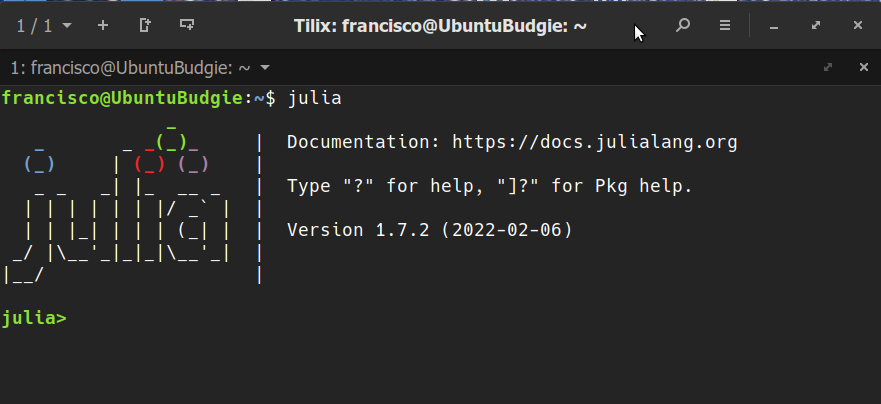
\includegraphics[width=0.65\textwidth]{fig/Julia_REPL} 
	\\(a)\\
	\vspace{1cm}
	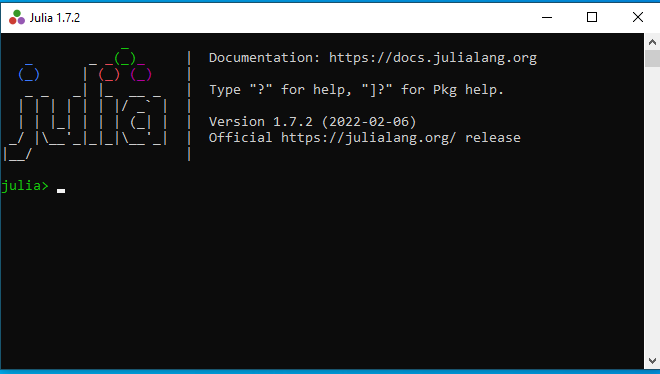
\includegraphics[width=0.65\textwidth]{fig/julia_in_windows}
	\\(b)\\
	\caption{Example of the REPL's welcome screen for Julia on a machine running Ubuntu Budgie (a) and Microsoft Windows (b).}
	\label{Fig;JuliaREPL}
\end{figure}
%
If no additional tool is installed, Julia will be executed in a REPL as it is shown in Fig. \ref{Fig;JuliaREPL}. However, most of the users prefer to use the language in conjunction with IDEs or notebooks such as:`

\begin{itemize}
	\item \textbf{Visual Studio Code}: Popular IDE developed by Microsoft with plugins for Julia. It can be downloaded from \href{https://code.visualstudio.com/}{https://code.visualstudio.com/} and the plugins installed as an extension. See \href{https://code.visualstudio.com/docs/languages/julia}{https://code.visualstudio.com/docs/languages/julia} for further information.
	%
	\item \textbf{Atom}: Just like VS Code, it is a general-purpose IDE with plugins for Julia. It can be downloaded from \href{https://atom.io/}{https://atom.io/}, with Julia plugins on \href{https://junolab.org/}{https://junolab.org/}. Thus, Atom becomes Juno, an IDE for Julia.
	%
	\item \textbf{Jupyter}: Although it is typically used for Python, it is also appropriate for Julia. Indeed, Jupyter is an acronym for \textbf{Ju}lia-\textbf{Pyth}on-\textbf{R}. There are different ways of installing Jupyter. In systems with Microsoft Windows OS, the most simple way is to install Anaconda \href{https://www.anaconda.com/products/individual}{https://www.anaconda.com/products/individual}. It can be setup to use Julia as calculation engine. In GNU/Linux there are smaller packages to install Jupyter. For example, in Ubuntu the simple instruction \texttt{sudo apt install jupyter-notebook} will install the software in your computer. Later, it is necessary to install an additional package inside Julia but this will be studied a bit later.
	
	Modern versions of Julia allow skipping this step, as we will see later. If not Jupyter is not found, Julia  downloads and locally installs the software.
	%
	\item \textbf{Pluto}: A notebook following the philosophy of Jupyter but specifically developed for Julia and easily extensible with JavaScript. Unlike the previous tools, it is installed inside Julia, not along with it. 
\end{itemize}
%
Atom, Jupyter and Pluto require the installation of additional packages to link Julia to the IDE. As Jupyter is probably the most popular tool, it is installed inside Julia REPL with the following instructions:

\vspace{1mm}
\begin{center}
	\texttt{using Pkg; Pkg.add("IJulia")}
\end{center}
\vspace{1mm}

This adds the package IJulia to the basic Julia installation. However, a previous step is to search for Jupyter on your computer. In the case of not finding it, Julia suggests to download a minimal version of Conda, thus installing Jupyter, as shown in Fig. \ref{Fig:Installling_Conda_with_julia}. Finally, it is launched  inside Julia as follows:
%
\begin{figure}
	\centering
	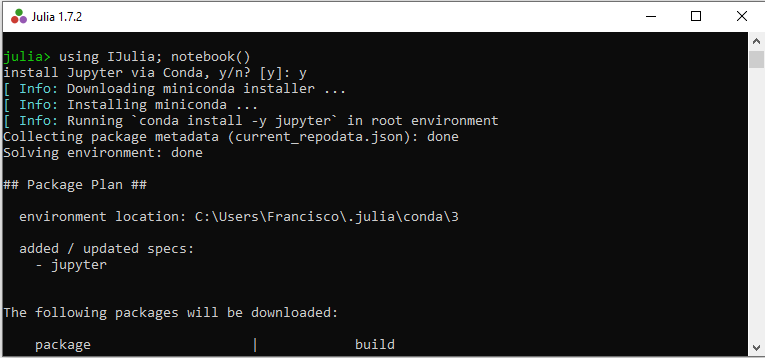
\includegraphics[width=0.65\textwidth]{fig/Julia_using_miniconda}
	\caption{If Jupyter is not detected, Julia installs a minimal version the first time IJulia is used.}
	\label{Fig:Installling_Conda_with_julia}
\end{figure}

\vspace{1mm}
	\begin{center}
		\texttt{using IJulia; notebook()} 
	\end{center}
\vspace{1mm}

Pluto package is installed following a similar procedure. 

\vspace{1mm}
\begin{center}
	\texttt{using Pkg; Pkg.add("Pluto");}
\end{center}
\vspace{1mm}

and launched with:

\vspace{1mm}
\begin{center}
	\texttt{using Pluto; Pluto.run()}
\end{center}
\vspace{1mm}

There are other options if you prefer cloud computing. For  example, in spite of the fact that its primary use is running Python code, Google Colab is compatible with Julia language. For further information (and also learning a little Julia), you can read \href{https://colab.research.google.com/github/ageron/julia_notebooks/blob/master/Julia_for_Pythonistas.ipynb#scrollTo=GIeFXS0F0zww}{Julia for Pythonists} and use the \href{https://colab.research.google.com/github/ageron/julia_notebooks/blob/master/Julia_Colab_Notebook_Template.ipynb}{Julia Colab Template}. However, this solution is not recommended due to some problems at installing external packages as well as at loading data files. Perhaps this flaw can be fixed in the future, but, nowadays, the tool is not as powerful as the others.

\section{Installing LELAPE}
LELAPE is built as a module. In Julia, a module is a set of elements such as variables, functions, etc. that can be loaded at will. The procedure is the following:
%
\begin{enumerate}
	\item Download the ZIP system from the website and decompress it. Also, you can clone the site with \texttt{git}. The instruction is \texttt{git clone https://github.com/fjfrancopelaez/LELAPE.git}.
	\item Find the \texttt{LELAPE/src} folder where a file called LELAPE.jl is located.
	\item Copy the full path pointing to this folder (\texttt{PATH\_TO\_FOLDER}) and execute in REPL, Jupyter or the notebook you use the following command:
	
	\vspace{1mm}
	\begin{center}
		\texttt{{push!(LOAD\_PATH,"PATH\_TO\_FOLDER")}}
	\end{center}
	\vspace{1mm}	
	
	For example, if LELAPE.jl is found in \texttt{/home/johndoe/Download/LELAPE/src/}, the instruction is:
		
	\vspace{1mm}
	\begin{center}
		\texttt{push!(LOAD\_PATH, "/home/johndoe/Download/LELAPE/src")}
	\end{center}
	\vspace{1mm}	
	
	Thus, Julia knows where to find the module. \texttt{LOAD\_PATH} is a string vector that contains the list of folder where Julia must look up external libraries. \texttt{push!} is a function that adds a new element at the end of any vector, keeping the name. Therefore, we have just added a new entry to the original list.	Fig. \ref{Fig:Loading_LELAPE} is a snapshot of the Julia terminal in GNU/Linux.
	%
	\begin{figure}
		\centering
		
		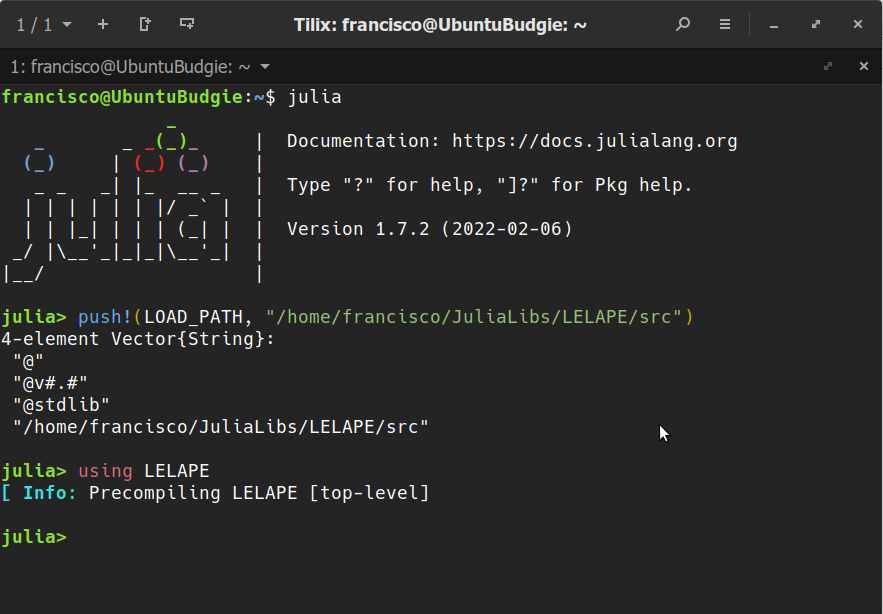
\includegraphics[width=0.65\textwidth]{fig/Loading_LELAP.png}
		\caption{How to indicate Julia where LELAPE is installed, and how to load it.}
		\label{Fig:Loading_LELAPE}
	\end{figure}
	
	A warning for users of Microsoft Windows: in this operating system, folders in the path are marked with the symbol \texttt{$\backslash$}. For technical reasons, this is not recognized in Julia, so the path to LELAPE must be modified with one of the following tips:
	%
	\begin{itemize}
		\item Replacing  \texttt{$\backslash$} with \texttt{/}, emulating the Unix style (GNU/Linux and Mac OS X).
		\item Replacing \texttt{$\backslash$} with \texttt{$\backslash\backslash$}.
	\end{itemize}
	%
	Fig. \ref{Fig:LELAPE_PATH_Windows} shows how to sucessfully add a new element to \texttt{LOAD\_PATH} with the first option\footnote{The instruction was \texttt{push!(LOAD\_PATH, "C:/Users/francisco/Desktop/LELAPE-main/LELAPE/src")}, although \texttt{push!(LOAD\_PATH, "C:{\textbackslash\textbackslash}Users{\textbackslash\textbackslash}francisco{\textbackslash\textbackslash}Desktop{\textbackslash\textbackslash}LELAPE-main{\textbackslash\textbackslash}LELAPE {\textbackslash\textbackslash}src")}}
	%
	\begin{figure}
		\centering
		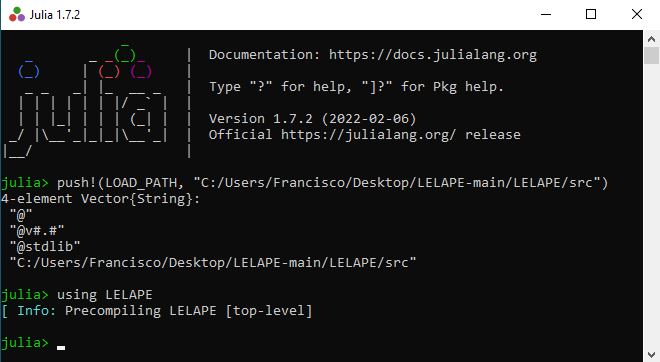
\includegraphics[width=0.65\textwidth]{fig/Julia_loading_LELAPE}
		\caption{The folder containing LELAPE is added to the admitted paths in Microsoft Windows.}
		\label{Fig:LELAPE_PATH_Windows}
	\end{figure} 

	\item Now, just launch LELAPE with the following instruction:
		
	\vspace{1mm}
	\begin{center}
		\texttt{using LELAPE}
	\end{center}
	\vspace{1mm}	
		
	After a few seconds to precompile the library, the functions are loaded. Figs. \ref{Fig:Loading_LELAPE} \& \ref{Fig:Julia_in_macoc} show practical examples.
\end{enumerate}

\begin{figure}
	\centering
	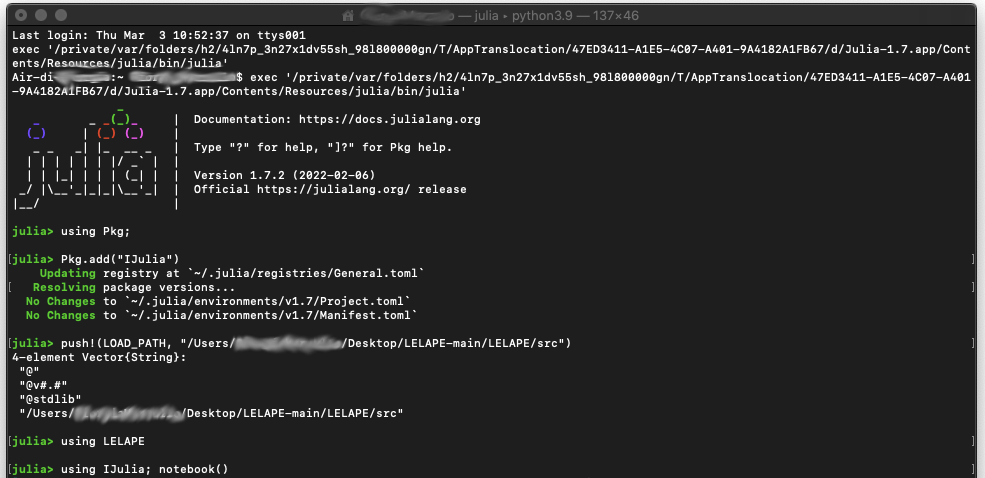
\includegraphics[width=0.65\textwidth]{fig/Julia_in_macOS_anonymous}
	\caption{Executing Julia on macOS and loading LELAPE.}
	\label{Fig:Julia_in_macoc}
\end{figure}

Jupyter users should be aware of a detail. Even if it is loaded on the terminal, it does not inherit loaded packages or modules, so they must be loaded again and independently in Jupyter. Even more, the \texttt{LOAD\_PATH} variable is initialized with its default value, with only three elements, so the instruction \texttt{push!(LOAD\_PATH, "PATH\_TO\_FOLDER")} must be executed again before loading LELAPE.

\section{Recommended packages}
%
There are many Julia packages at the user's disposal that can be found on \href{https://juliapackages.com/}{https:// juliapackages.com/}. Some packages are extremely popular:
\begin{itemize}
	\item \textbf{Revise}: Useful for code developers since it allows reloading user functions without restarting Julia and losing information.
	\item \textbf{OhMyREPL}: Inteligent highlighting of elements in REPL. Figs. \ref{Fig;JuliaREPL} \& \ref{Fig:Loading_LELAPE} are using this package to show function names and strings.
\end{itemize}

Both are installed with \texttt{Pkg.add()}. 

Another interesting package to have is \textbf{DelimitedFiles}, which allows reading and writing CSV files. It is an essential package in Julia, available in a fresh installation, but not loaded by default. It is not necessary to fetch it and it is loaded as:
	
\vspace{1mm}
\begin{center}
	\texttt{using DelimitedFiles}
\end{center}
\vspace{1mm}	

This package is necessary to use the illustrative Jupyter notebooks that are provided along with LELAPE.

\textbf{A tip for new users}: after working with Julia for a long time, you may eventually discover that only a few packages are frequently used and  you may get bored of loading them every time you start a new session. Thus, the typical solution is to create the following folder and text file in your home directory:
%
\begin{itemize}
	\item In GNU/Linux \& Mac OS X: \texttt{/home/<USER>/.julia/config/startup.jl}
	\item In Microsoft Windows: \texttt{C:{\textbackslash}Users{\textbackslash}<USER>{\textbackslash}.julia{\textbackslash}config{\textbackslash}startup.jl}
\end{itemize}  
%
Fig. \ref{Fig:startup.jl} is an example of the \texttt{startup.jl}. In this file, one can see that LELAPE placement is automatically loaded when the session begins. However, if you wish to load these packages in Jupyter, it is necessary to create a new file, \texttt{startup\_ijulia.jl}, with identical information. However, a soft link to \texttt{startup.jl} is enough.
%
\begin{figure}
	\centering
	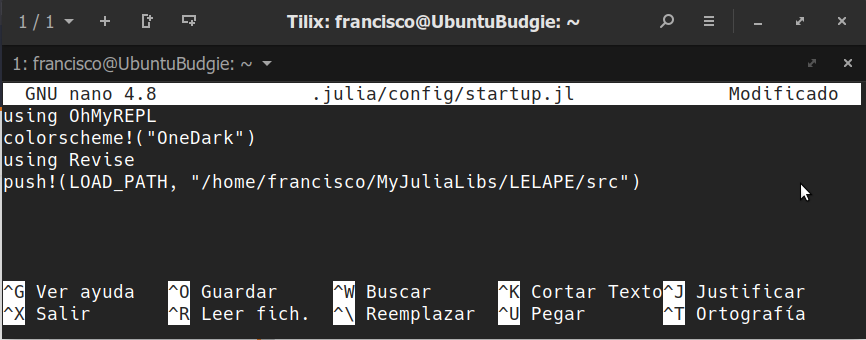
\includegraphics[width=0.65\textwidth]{fig/startup.jl}
	\caption{Example of \texttt{startup.jl} file in GNU/Linux.}
	\label{Fig:startup.jl}
\end{figure} 
\chapter{How to use LELAPE}
\section{Formatting input data}
%
You are supposed to have performed experiments on some memory element. Tests were performed as:
\begin{itemize}
	\item \textbf{Static}: The device was written, sent to standby mode, irradiated and eventually read. The content after the irradiation was compared to the initially writing.
	\item \textbf{Pseudostatic}: Similar to static ones, but standby intervals are shorter than the irradiation time and the memory is read several times during the irradiation. Usually, flipped bits are corrected on the fly \cite{Gupta2017}.
	\item \textbf{Dynamic}: A typical experiment consists in performing a continuous reading \& writing process while the memory is irradiated with a predefined algorithm to detect failures \cite{Tsiligiannis2014a, Tsiligiannis2014b}. 
\end{itemize}

In any of these cases, the researcher saves information about the bitfilps: Word address, read content, initial pattern, ... 
In order to use LELAPE, radiation test data must be converted to a matrix with three or four columns. The meaning of the columns is the following:
\begin{itemize}
	\item \textit{First Column}: Word Address where bitflips were observed.
	\item \textit{Second Column}: Content in the word address after the radiation tests.
	\item \textit{Third Column}: Content in the word address before the irradiation.
	\item \textit{Fourth Column}: In pseudostatic tests, cycle in which the bitflip was observed. This column can be omitted in the static tests or replaced by a column full of ones.  
	
	This calumn is also necessary for dynamic tests. In each step of the algorithm, the memory is fully explored and the discrepancies registered. So, in practice, for analysis with LELAPE the only differences between dynamic and psedostatic tests are that, in the former, the pattern changes from cycle to cycle, and that the addresses are recorded in different orders, sometimes increasing, sometimes decreasing, etc. These details are irrelevant for the tool.
\end{itemize} 

LELAPE needs this elements to be converted to a UInt32 matrix\footnote{In Julia, typing variable is optional but encouraged to speed up calculations.} so it is important that all the elements of the matrix, including the cycle label, are in this format or, at least, in some kind of integer. This makes dangerous labelling the fourth column with words or letters. 

A simple solution consists in grouping the data results in CSV format and read this text file with \texttt{readdlm}, included in the \text{DelimitedFiles} package. In the Jupyter folder, you can see some examples that can guide you to adapt your own data. One advantage of this function is that it can automatically convert the data to the required format, as shown in the Jupyter notebooks.

\section{Setting up the analysis}
%
Before starting the analysis, we must define some additional variables to indicate the software how to proceed. These variables are the followong:
%
\begin{itemize}
	\item \textbf{LA}: Variable in integer format. It indicates the memory size in words (not in bits!). It is often a power of 2.
	\item \textbf{WordWidth}: Also an integer, it indicates the number of bits per word. Typically 8, 16, 32 but other values are possible.
	
	If you had registered your data directly with the cell address, disregarding any organization in words, just set \texttt{WordWidth = 1} and \texttt{LA  = \(L_N\)}, this being the memory size in bits.
	
	\item \textbf{Operation}: A string variable to indicate the mathematical operation used to create the DV set. So far, only two options are implemented:
	\begin{itemize}
		\item \textit{XOR}: Addresses are xored bit to bit. This mode is set with the \texttt{"XOR"} value.
		\item \textit{Positive subtraction}: The absolute value of the difference of addresses is returned. It is marked with \texttt{"POS"}. 
	\end{itemize}

	In practice, we have observed that the former is appropriate for SRAMs and the latter for FPGAs. However, this idea may be erroneous due to the use of few and partial radiation test data.
	%
	\item \textbf{UsePseudoAddress}: The pseudoaddress is defined as follows: let us suppose that we have observed a bitflip in the $k$-th position of the $NWA$-th word address, The word width is $W$ and $k=0$ corresponds to the least significant bit, $W-1$ to the most significant one. Hence, the pseudoaddress of the bitflip is:
	%
	\begin{equation}
		PSA = NWA \cdot W + k
		\label{Eq:PseudoAddress}
	\end{equation}
	%
	This value is full of meaning in FPGAs since just returns the position of the cell in the bitflips. It is completly artificial in some SRAMs but somehow analysis using the pseudoaddress instead of the word address are more accurate and efficient. 
	
	The researcher can set this variable to \texttt{true} or \texttt{false} at will.
	%
	\item \textbf{KeepCycles}: In pseudostatic tests, this boolean variable indicates that the system must use the information about the cycles (fourth column) or just using the set of data as a whole. 
	
	Before going on, a little tip to treat data from\textbf{ field tests} where a large number of similar devices are exposed to natural radiation. An option to analyze data would have been define a new pseudoaddress adding the position of the device in the bank, \(k_{MEM}\), and the memory size in bits, \(L_N\):
	\[
		PSA^* = k_{MEM}\cdot L_N + NWA \cdot W + k
	\]
	This may work, but is strongly computationally inefficient for LELAPE. Instead of it, we recommend to redefine the reading cycle index. Let us suppose that there are \(N_{MEM}\) identical memories in the bank, and that they are indexed from \(k_{MEM}=0\) to \(k_{MEM}=N_{MEM}-1\). If the bank reading cycle is \(k_{BNK}\), the cycle to be included in the CSV file should be:
	%
	\begin{equation}
		Cycle = k_{BNK}\cdot N_{MEM}+k_{MEM}
	\end{equation}
	%
	In other words, we are redefining cycles at device level, not bank level. This solution is much more efficient for LELAPE.
	%
	\item \textbf{TraceRuleLength}: This an integer variable with 1,2 or 3 as allowed values. LELAPE looks for anomalously repeated elements in the DV set with very few ones in binary representation. The user can decide if looks for elements with 1, 2 or 3 ones or less and include them as candidates to detect pairs. 
	%
	\item \textbf{$\varepsilon$}: A float number always positive but close to 0. If the expected number of elements repeated $k$ times in the DV set is lower than $\varepsilon$, we must consider this number of repetitions impossible. If higher, we determine than at least an element can appear $k$ times just due to randomness. Default value is 0.05.
	
	A very low value of $\varepsilon$ will exclude false positive but also genuine values relating pair of addresses in an MCU. On the contrary, if it is chosen too low, false positives might be taken as good ones.
	%
	\item \textbf{LargestMCUSize}: During the search of critical DV values, LELAPE starts to group addresses in provisional MCUs that grow large and large as new possible critical DV values are tested. Unfortunately, sometimes this process does not find a stable solution and goes on looking for it despite being unrealistic. This parameter is used to stop the calculation since it informs the software of not considering MCUs with more than \textit{LargestMCUSize} addresses. By default, it is set to 200, but, if you do not expect such a large event, reduce its value in order to unburden the computer memory usage. 
\end{itemize}

 \section{Functions in the module}
 %
 The functions depicted in this section are included in LELAPE and also accessible from the REPL, Jupyter, etc. Other functions are for internal use in LELAPE and are excluded from this list. The reader can just open the individual \texttt{.jl} files and check the comments.
 
 Available functions are grouped in several categories:
 \begin{itemize}
 	\item \hyperref[SubseC:PreparationExpdata]{Preparation of experimental data}
 	\item \hyperref[SubSeC:MBUs]{Multiple Bit Upsets}
 	\item \hyperref[Subsec:StatisticalPredictions]{Statistical predictions}
 	\item \hyperref[Subsec:SearchOfAnomalies]{Search of anomalies}
 	\item \hyperref [SubSec:ClassificationEventsFromAnomalies]{Classification of events from anomalies}
 	\item \hyperref[SubSec:FalseEvents]{False events due to accumulation of bitflips}
 \end{itemize}
 %
 In all the items you will find the accepted input arguments, the kind of output as well as an explication of its purpose.
 %
 \subsection{Preparation of experimental data}\label{SubseC:PreparationExpdata}
 %
 These functions just adapt the original test data to be used by LELAPE, or provide information about the data set. In this section, the following functions are included:
 \begin{itemize}
 	\item \hyperref[Func:ConvertToPseudoADD]{ConvertToPseudoADD}
 	\item \hyperref[Func:AddPatternColumn]{AddPatternColumn}
 	\item \hyperref[Func:ExtractFlippedBits]{ExtractFlippedBits}
 	\item \hyperref[Func:Npairs]{Npairs}
 	\item \hyperref[Func:NTriplets]{NTriplets}
 \end{itemize}
 %
 \subsubsection*{ConvertToPseudoADD}\label{Func:ConvertToPseudoADD}
 \begin{itemize}
 	\item \textbf{Input arguments}: 
 	\begin{itemize}
 		\item \textit{Method 1: }\textbf{DATA}::Array\{UInt32\}, \textbf{WordWidth}::Int
 		\item \textit{Method 2: }\textbf{DATA}::Array\{UInt32\}, \textbf{WordWidth}::Int, \textbf{KeepCycle}::Bool
 	\end{itemize}
 
 	In the case of not providing \textbf{KeepCycle}, it is assumed to be \texttt{false}.
 
 	\item   \textbf{Output}: Array\{UInt32, 2\}, or Matrix\{UInt32\}.
 	\item  This function looks for the flipped bits between words in the same row but in the second
 	and third columns of the \textbf{DATA} matrix. It does not matter if there are several bitflips, since they are independently counted. 
 	The pseudoaddress  of each bitflip, defined as \[\text{WORDADDRESS}\times\text{Wordwith}+\text{Bitposition}\] (Eq. \ref{Eq:PseudoAddressDefinition}) is returned as the first column of the output.
 
 	If there is information about the different cycles, it can be kept in the optional second column in the output with the condition of previously declaring \textbf{KeepCycle} as true. If cycle information is absent, the second column is filled with 1's.
 	
 	Fig. \ref{fig:Example_ConvertToPseudoADD} shows an example of use in the REPL. There are more rows in the output matrix than in the input one since there are words with several flipped bits.
 	
 	\begin{figure}[h!]
 		\centering
 		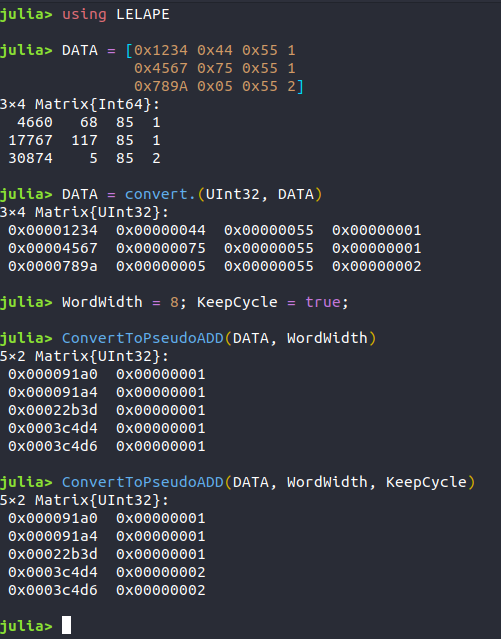
\includegraphics[width=0.65\columnwidth]{fig/functions/ConvertToPsudoADD.png}
 		\caption{Example of use of \texttt{ConvertToPseudoADD}.}
 		\label{fig:Example_ConvertToPseudoADD}
 	\end{figure}
 \end{itemize}
%
 \subsubsection*{AddPatternColumn}\label{Func:AddPatternColumn}
 
 TBD
 
 \subsubsection*{ExtractFlippedBits}\label{Func:ExtractFlippedBits}
 \begin {itemize}
 \item \textbf{Input arguments}:
 \begin{itemize}
 	\item \textit{Method 1: }\textbf{WORD}::UInt32, \textbf{PATTERN}::UInt32, \textbf{Wordwidth}::Int
 	\item \textit{Method 2: }\textbf{WORD}::UInt16, \textbf{PATTERN}::UInt16, \textbf{Wordwidth}::Int
 	\item \textit{Method 3: }\textbf{WORD}::UInt8, \textbf{PATTERN}::UInt8, \textbf{Wordwidth}::Int
 \end{itemize}
 \item \textbf{Output}: :Array\{Int,1\}, or Vector\{Int\}
 \item This function allows discovering the position of different bits between \textbf{WORD}
 and \textbf{PATTERN}. It also verifies that both values are coherent with the \textbf{Wordwidth},
 meaning that neither of them are higher than \(2^{Wordwidth}-1\). A vector, never larger than \textbf{Wordwidth} is returned. If this condition is not fulfilled, the functions returns an error. If \textbf{WORD} and \textbf{PATTERN} are equal, the output is a void vector.
 %
 \begin{figure}[h!]
 	\centering
 	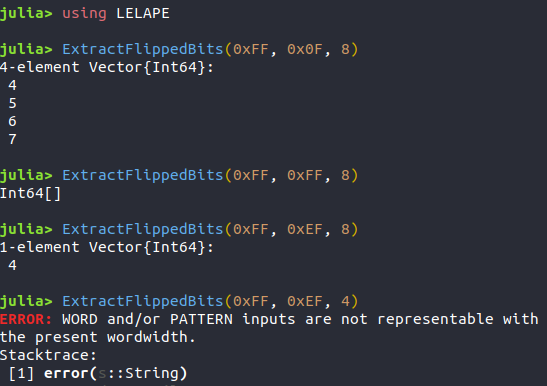
\includegraphics[width=0.65\columnwidth]{fig/functions/ExtractFlippedBits.png}
 	\caption{Example of use of \texttt{ExtractFlippedBits}.}
 	\label{fig:Example_ExtractFlippedBits}
 \end{figure}
 
 Fig. \ref{fig:Example_ExtractFlippedBits} shows some examples of use of this function. Take into account that, even when there is a single bitflip, a vector is always returned, albeit with an only value inside.
\end{itemize}
%
\subsubsection*{NPairs}\label{Func:Npairs}
\begin{itemize}
	\item \textbf{Input arguments}:
	\begin{itemize}
		\item \textit{Method 1}: \textbf{DATA}::Array{UInt32}
		\item \textit{Method 2}: \textbf{DATA}::Array{UInt32}, \textbf{UsePseudoAdd}::Bool
		\item \textit{Method 3}: \textbf{DATA}:: Array{UInt32}, \textbf{UsePseudoAdd}::Bool, \textbf{WordWidth}:: Int
		\item \textit{Method 4}: \textbf{DATA}::Array{UInt32}, \textbf{UsePseudoAdd}:: Bool, \textbf{WordWidth}:: Int, \textbf{KeepCycle}:: Bool
		\item \textit{Method 5}: \textbf{N}::Int
	\end{itemize}

	In Methods 1--4, default values for parameters are \texttt{\textbf{UsePseudoAdd} = false}, \texttt{\textbf{WordWidth} = 1}, \texttt{\textbf{KeepCycle} = false}. 
	
	\item \textbf{Output}: Int 
	%
	\item \textbf{DATA} is a 3 or 4-column matrix derived from the loaded CSV file and each row containing the word address (\#1), the read word after the tests (\#2), the initial pattern (\#3) and the number of reading cycle when the error was observed. If this last column is not provided or \textbf{KeepCycle} is false, the system works as if only one cycle was done. 
	
	The function provides the number of pairs of addresses taken during each cycle regarding predictions of the Only-SBU model (Eq. \ref{Eq:SizeOfDV}). For example, let us suppose that we have done 2 cycles, observing in the first one 30 events, and 40 in the second. The number of possible pairs is the addition of the pairs in each cycle:
	\[
	\frac{1}{2}\cdot 30\cdot(30-1)+\frac{1}{2}\cdot 40\cdot(40-1) = 1215
	\]
	Thus, 1215 pairs can be formed. If we had not taken into account the existence of cycles, the number of pairs would have been\[	\frac{1}{2}\cdot (30+40)\cdot(30+40-1) = 2415\]
	however, many of them are unreal since were taken in different times!
	
	If \textbf{UsePseudoAdd} is set to true, the system looks for the position of the bitflips inside the word and uses the pseudoaddress (\(\text{WordAddress}\times\text{WordWidth}+\text{Position}\)). Thus, it is necessary to provide the \textbf{WordWidth} value (8, 16, 32, ...). Using \textbf{DATA} as the only argument is appropriate to analyze values directly in pseudoaddress format (or just the word address) taken during one only cycle. This is the case, for example, of FPGAs configuration memory. 
	
	There is a final method, just saying the number of observed pairs, \textbf{N}. In this case, the function returns \textbf{N}\(\cdot\)(\textbf{N}-1)/2.

	\begin{figure}[h!]
		\centering
		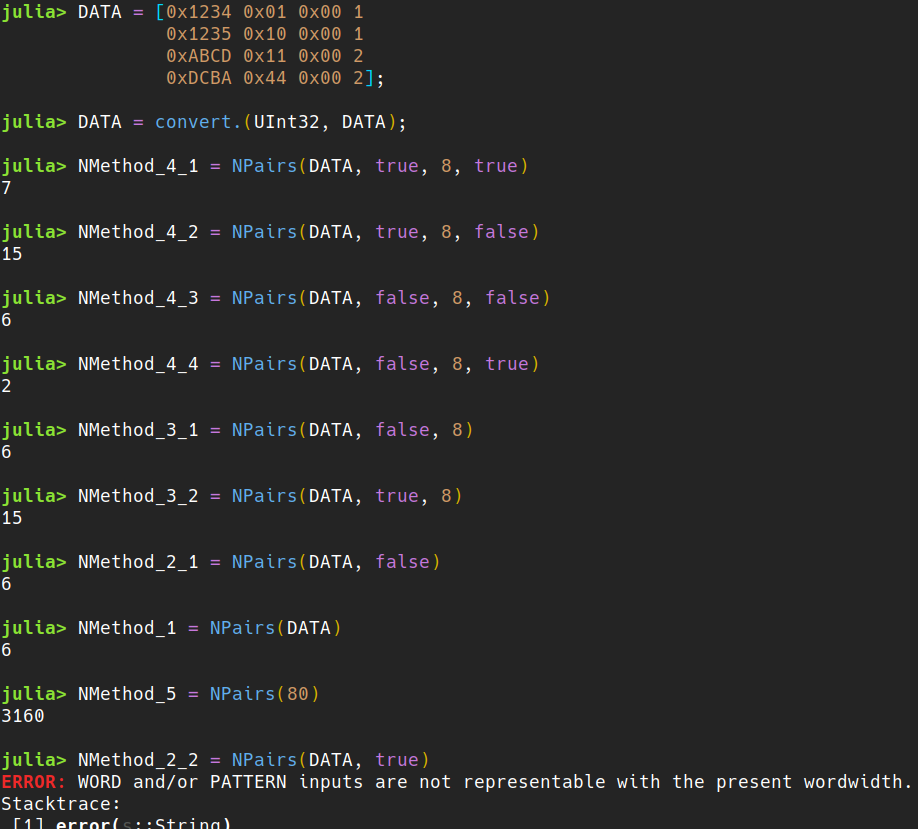
\includegraphics[width=0.75\columnwidth]{fig/functions/NPairs.png}
		\caption{Example of use of \texttt{NPairs}.}
		\label{fig:Example_NPAirs}
	\end{figure}

	Fig. \ref{fig:Example_NPAirs} shows an example of use of this function. 
	
\end{itemize}
%
\subsubsection*{NTriplets}\label{Func:NTriplets}
\begin{itemize}
	\item \textbf{Input arguments}:
	\begin{itemize}
		\item \textit{Method 1}: \textbf{DATA}::Array{UInt32}
		\item \textit{Method 2}: \textbf{DATA}::Array{UInt32}, \textbf{UsePseudoAdd}::Bool
		\item \textit{Method 3}: \textbf{DATA}:: Array{UInt32}, \textbf{UsePseudoAdd}::Bool, \textbf{WordWidth}:: Int
		\item \textit{Method 4}: \textbf{DATA}::Array{UInt32}, \textbf{UsePseudoAdd}:: Bool, \textbf{WordWidth}:: Int, \textbf{KeepCycle}:: Bool
		\item \textit{Method 5}: \textbf{N}::Int
	\end{itemize}
	\item \textbf{Output}: Int
	%
	\item Similar to \textit{Npairs(...)}, but calculating the expected number of triplets instead of pairs. Thus, instead of using Eq. \ref{Eq:SizeOfDV} as the basis for calculations, this function uses:
	\[
		N_{Triplets} = \frac{1}{6}\cdot N_{BF}\cdot \left(N_{BF}-1\right)\cdot \left(N_{BF}-2\right)
	\]
\end{itemize}
%
\subsection{Multiple Bit Upsets} \label{SubSeC:MBUs}
%
Sometimes, the researcher just wants to know how many multiple bit upsets occurred during the experiments. There is only one function in this section, \texttt{CheckMBUs}.

\subsubsection*{CheckMBUs}

\begin{itemize}
	\item \textbf{Input arguments}:
	\begin{itemize}
		\item \textit{Method 1}: \textbf{WORD}::UInt32, \textbf{PATTERN}::UInt32, \textbf{WordWidth}::Int
		\item \textit{Method 2}: \textbf{WORDS}::Vector\{UInt32\}, \textbf{PATTERN}::Vector\{UInt32\}, \textbf{WordWidth}::Int
		\item \textit{Method 3}:  \textbf{WORDS}::Vector\{UInt32\}, \textbf{PATTERN}::UInt32, \textbf{WordWidth}::Int
	\end{itemize}
	\item \textbf{Output}: 
		\begin{itemize}
			\item \textit{Method 1}: Tuple\{Int, Vector\{Int\}\}
			\item \textit{Methods 2 \& 3}: Tuple\{Vector\{Int\}, Vector\{Any\}\}
		\end{itemize}
	%
	\item The first method is quite easy to understad. It just takes to unsigned integer 32-bit numbers, \textbf{WORD} \& \textbf{PATTERN}, of which only the last \textbf{WordWidth} bits are significant, and looks for equivalent bits with different value with the function \hyperref[Func:ExtractFlippedBits]{\texttt{ExtractFlippedBits}}. Then, it returns the number of biflips and a vector containing the flipped positions. Fig. \ref{fig:Example_CheckMBUs_M1} shows how this function behaves with these inputs.
	
	\begin{figure}[h!]
		\centering
		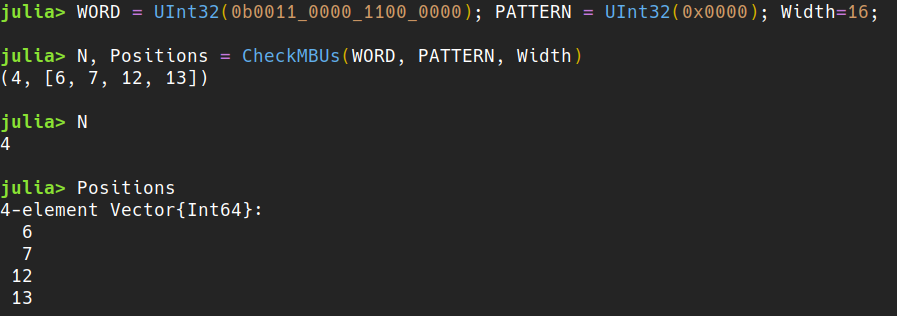
\includegraphics[width=0.75\columnwidth]{fig/functions/CheckMBUs_M1.png}
		\caption{Example of use of \texttt{CheckMBUs} with unsigned integers as inputs.}
		\label{fig:Example_CheckMBUs_M1}
	\end{figure}

	For Method 2, the idea is to provide as arguments two similar-length vectors with the \textbf{WORD} and \textbf{PATTERN} values in UInt32 format, as well as the \textbf{WordWidth}. Then, the function checks the values in both vectors with the same index and returns two vectors. The first one is a typical vector of integers, containing in the \(k\)-th position the number of different bits between \textbf{WORD}[k] y \textbf{PATTERN}[k]. The second is a vector of vectors. Thus, the element in the \(k\)-th positiion is also a vector with the positions of the flipped bits. 
	
	Method 3 is quite similar to Method 2, but \textbf{PATTERN} is no longer a vector but a constant value for all the elements of \textbf{WORDS}. Fig. \ref{fig:Example_CheckMBUs_M23} shows how this method and the previous one work.
	
	\begin{figure}[h!]
		\centering
		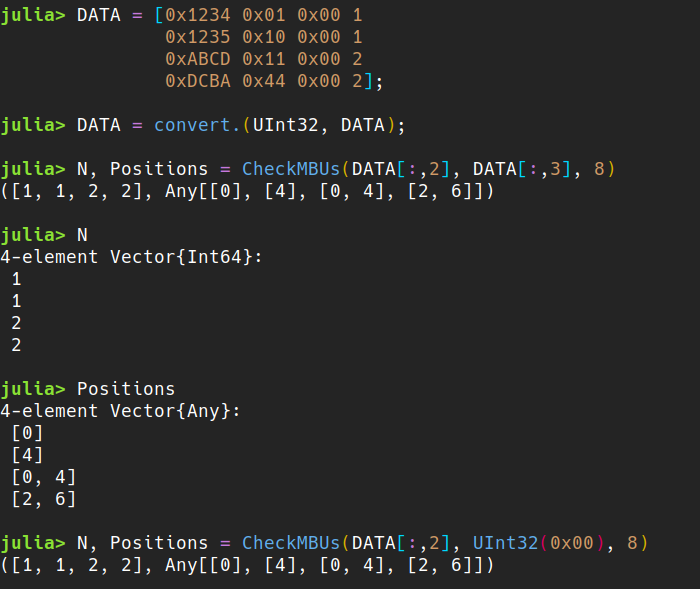
\includegraphics[width=0.75\columnwidth]{fig/functions/CheckMBUs_Methods2_3.png}
		\caption{Example of use of \texttt{CheckMBUs} with vectors as inputs. Last line uses Method 3, where the pattern is provided as an unsigned integer.}
		\label{fig:Example_CheckMBUs_M23}
	\end{figure}
	
\end{itemize}
%
\subsection{Statistical predictions}\label{Subsec:StatisticalPredictions}
%
The goals of this set of functions is to cast predictions about the characteristics of the data according to the Only-SBU model. The following functions are included in this section:

\begin{itemize}
	\item \hyperref[Subsec:MaxExpectedRepetitions]{MaxExpectedRepetitions}
	\item \hyperref[Subsec:TheoAbundance_POS]{TheoAbundance\_POS}
	\item \hyperref[Subsec:TheoAbundance_XOR]{TheoAbundance\_XOR}
	\item \hyperref[Subsec:TheoAbundance]{TheoAbundance}
\end{itemize}

Related to these functions are those used to determine the expected number of false errors, but they will be depicted in the corresponding section.
%
\subsubsection*{MaxExpectedRepetitions}\label{Subsec:MaxExpectedRepetitions}
%
\begin{itemize}
	\item \textbf{Input arguments}: 
	\begin{itemize}
		\item \textit{Method 1}: \textbf{NDV}::Int, \textbf{LN}::Int, \textbf{Operation}:: String, \(\varepsilon\):: AbstractFloat	
		\item \textit{Method 2}: \textbf{NDV}::Int, \textbf{LN}::Int, \textbf{Operation}::String
	\end{itemize}
	\item \textbf{Output}: Int
	\item The purpose of this funcion is to determine the maximum number of expected
	repetitions. in a DV set taken from a memory with size equal to \textbf{LN} .
	In general, it is the first integer such that its theoretical abundance is
	lower than \(\varepsilon\). If this threshold is not provided, it is assumed to be \(\varepsilon = 0.01\).
\end{itemize}
%
\subsubsection*{TheoAbundance\_POS}\label{Subsec:TheoAbundance_POS}
%
\begin{itemize}
	\item \textbf{Input arguments}:
	%
	\begin{itemize}
		\item \textit{Method 1}: \textbf{NR}: :Int, \textbf{NB}::Int, \textbf{LN}::Int, \textbf{UsingDV}::Bool
		\item \textit{Method 2}: \textbf{NR}: :Int, \textbf{NB}::Int, \textbf{LN}::Int
	\end{itemize}
	\item \textbf{Output:} AbstractFloat
	%
	\item This function allows calculating the expected number of values repeated 	 \textbf{NR} times after several bitflips in a memory with \textbf{LA} words with \textbf{W} bits per word   	supposing to have used the POSITIVE subtraction.
	
	\textbf{NR} must be an integer number higher than or equal to 0. 
	\textbf{NB} is an integer number supposed to be higher than 1.
	\textbf{LN} is an integer number, and indicates the size of the memory. If the researcher uses bit address for calculations, \textbf{LN} is \textbf{LA}\(\times\)\textbf{W}. However, if he/she uses the word address instead, this parameerter is \textbf{LA}.
	
	\textbf{UsingDV} determines how \textbf{NB} must be interpreted. If that boolean variable is \texttt{true}, \textbf{NB} is the size of the DV set, called elsewhere \(N_{DV}\). If false, \textbf{NB} is the number of bitflips and \(N_{DV}\) must be calculated from it. By default, \textbf{UsingDV} is \texttt{false}.
	
	Equations were got from Eq.2 of the Appendix in J. C. Fabero et al., "\textit{Single Event Upsets Under 14-MeV Neutrons in a 28-nm
		SRAM-Based FPGA in Static Mode,}" in IEEE Transactions on Nuclear Science, vol.
	67, no. 7, pp. 1461-1469, July 2020, doi: 10.1109/TNS.2020.2977874.
	
	Lawfully avalaible for free download on \href{https://eprints.ucm.es/id/eprint/59496/}{https://eprints.ucm.es/id/eprint/59496/}
\end{itemize}

\subsubsection*{TheoAbundance\_XOR}\label{Subsec:TheoAbundance_XOR}
%
\begin{itemize}
	\item \textbf{Arguments:}
	%
	\begin{itemize}
		\item \textit{Method 1}: \textbf{NR}: :Int, \textbf{NB}::Int, \textbf{LN}::Int, \textbf{UsingDV}::Bool
		\item \textit{Method 2}: \textbf{NR}: :Int, \textbf{NB}::Int, \textbf{LN}::Int
	\end{itemize}
	\item \textbf{Output:} AbstractFloat
	%
	\item Equivalent to \hyperref[Subsec:TheoAbundance_POS]{\texttt{TheoAbundance\_POS}}, but referred to the bitwise XOR operation. 
	
	Equations were got from Eq.12 of the Appendix.C in 
	F. J. Franco et al., "\textit{Statistical Deviations From the Theoretical Only-SBU
		Model to Estimate MCU Rates in SRAMs,}" in IEEE Transactions on Nuclear
	Science, vol. 64, no. 8, pp. 2152-2160, Aug. 2017,
	doi: 10.1109/TNS.2017.2726938. 
	
	Lawfully avalaible for free on https://eprints.ucm.es/id/eprint/43874/
\end{itemize}
%
\subsubsection*{TheoAbundance}\label{Subsec:TheoAbundance}
%
\begin{itemize}
	\item \textbf{Input arguments}:
	\begin{itemize}
		\item \textit{Method 1:} \textbf{NR}::Int, \textbf{NB}::Int, \textbf{LN}::Int, \textbf{Operation}:: String, \textbf{UsingDV}::Bool
		\item \textit{Method 1:} \textbf{NR}::Int, \textbf{NB}::Int, \textbf{LN}::Int, \textbf{Operation}:: String
	\end{itemize}
	\item \textbf{Output}: AbstractFloat
	\item This is an Alias for \hyperref[Subsec:TheoAbundance_POS]{ \texttt{TheoAbundance\_POS()}} or \hyperref[Subsec:TheoAbundance_XOR]{ \texttt{TheoAbundance\_XOR()}}. The definition of arguments are similar, with an additional parameter, \textbf{Operation}, which only can be \texttt{"XOR"} or \texttt{"POS"}. 
	
\end{itemize}
%%

%%%%%%%%%%%%%%%%%%%%%%%%5
\subsection{Search of anomalies}\label{Subsec:SearchOfAnomalies}

This is an important set of functions that determine the statistical anomalies in the data set, and discard those that are not trustworthy, perhaps due to interaction between events. 

The functions included in this section are:

\begin{itemize}
	\item  \hyperref[Fun:DetectAnomaliesSelfConsis]{DetectAnomalies\_SelfConsis}
	\item  \hyperref[Fun:DetectAnomaliesShuffleRule]{DetectAnomalies\_Shuffle\_Rule}
	\item  \hyperref[Fun:DetectAnomaliesTraceRule]{DetectAnomalies\_Trace\_Rule}
	\item  \hyperref[Fun:DetectAnomaliesMCURule]{DetectAnomalies\_MCU\_Rule}
	\item  \hyperref[Fun:DetectAnomaliesFullCheck]{DetectAnomalies\_FullCheck}
\end{itemize}

Last function just calls the previous four.

\subsubsection*{DetectAnomalies\_SelfConsis}\label{Fun:DetectAnomaliesSelfConsis}
\begin{itemize}
	\item \textbf{Input arguments}:
	\begin{itemize}
		\item  \textit{Method 1: }\textbf{DATA}::Array\{UInt32, 2\}, 
		\textbf{WordWidth}::Int,
		\textbf{LN0}::Int,
		\textbf{Operation}::String,
		\textbf{UsePseudoADD}::Bool,
		\textbf{KeepCycle}::Bool,
		\textbf{\(\varepsilon\)}::AbstractFloat,
		\textbf{LargestMCUSize}::Int
		%
		\item  \textit{Method 2: }\textbf{DATA}::Array\{UInt32, 2\}, 
		\textbf{WordWidth}::Int,
		\textbf{LN0}::Int,
		\textbf{Operation}::String,
		\textbf{UsePseudoADD}::Bool,
		\textbf{KeepCycle}::Bool,
		\textbf{\(\varepsilon\)}::AbstractFloat
		%
		\item  \textit{Method 3: }\textbf{DATA}::Array{UInt32, 2}, 
		\textbf{WordWidth}::Int,
		\textbf{LN0}::Int,
		\textbf{Operation}::String,
		\textbf{UsePseudoADD}::Bool,
		\textbf{KeepCycle}::Bool
	\end{itemize}

	Default values for \textbf{\(\varepsilon\)} \& 	\textbf{LargestMCUSize} are \texttt{0.05} and \texttt{200} respectively.
	%
	\item \textbf{Output: } Array\{UInt32, 2\}	
	%
	\item This function will calculate the anomalies in the set of addresses using \hyperref[Subsec:SelfConsistencyRule]{the Self Consistency rule}. 
	 First of all, let us know the inputs:
	 \begin{itemize}
	
		\item   \textbf{DATA}: A matrix with 3 or 4 columns. 
			 \begin{itemize}
			 	\item The first column contains the word addresses in UInt32 format.
			 	\item The second one shows the content read in the memory after the irradiation.
			 	\item The third one, the pattern that should be inside.
			 	\item  The fourth one is optional and shows the number of the read cycle if the   memory was read and corrected several times during the irradiation.
			 \end{itemize}
		\item   \textbf{WordWidth}: The size of each word in bits, usually 8, 16. 32, etc. No default value is provided.
		\item   \textbf{LN0}: The memory size in words (not in bits!!!). In many cases, a natural power of 2.
		\item   \textbf{Operation}: A string variable to indicate the preferred operation to calculate
	    the DV set. Only two operations are allowed: 
	    \begin{itemize}
	    	\item \texttt{"XOR"}: bitwise XOR.
	    	\item\texttt{ "POS"}: positive subtraction
	    \end{itemize}
		\item  \textbf{UsePseudoADD}: A boolean variable. Its purpose is to indicate that the user wants to use the word addresses when this parameter is false). If true, the pseudoaddress, calculated
	    as \(\text{WORADDRESS}\times\text{WordWidth} + \text{BitPosition}\), is used instead. Full of sense in FPGA since it is just the position  of the bit in the bitstream, it has not physical interpretation in memories BUT works!!!!
		\item   \textbf{KeepCycle}: If true, the function looks for the fourth column and uses it to calculate the DV Set.
		\item   \textbf{\(\varepsilon\)}: A small positive integer number to determine the threshold that defines when a number of repetitions are impossible to occur. Set by default to 0.05 if not provided among the input arguments.
		\item  \textbf{LargestMCUSize}: This value indicates the largest possible size for MCUs. It has not physical sense  and is only used to stop the program if unrealistic events occur. Set to 200 if not given as an input.

	\end{itemize}
	
	The function returns an \(N\times 2\) UInt32 matrix. The first column contains the anomalously repeated values of the DV SET compatible with the Self Consistency test. The second one contains the number of times they appear in the DV set. Due to format integrity reasons, this column is expressed in unnatural \texttt{UInt32} format. 
	
	It is advisable a latter conversion into Int to make this column more readable. There are several examples of this function or equivalent in the Jupyter folder.
	
	If the function does not find any anomaly, it returns a void matrix.  Or, more exactly, a \(0\times 2\) one.
\end{itemize}
%
\subsubsection*{DetectAnomalies\_Shuffle\_Rule}\label{Fun:DetectAnomaliesShuffleRule}
 TBD
 %
 \subsubsection*{DetectAnomalies\_Trace\_Rule}\label{Fun:DetectAnomaliesTraceRule}
 %
 TBD
 %
 \subsubsection*{DetectAnomalies\_MCU\_Rule}\label{Fun:DetectAnomaliesMCURule}
 %
 TBD
 %
 \subsubsection*{DetectAnomalies\_FullCheck}\label{Fun:DetectAnomaliesFullCheck}
 %
 TBD
 %
 \subsection{Classification of events from anomalies}\label{SubSec:ClassificationEventsFromAnomalies}
 \subsubsection*{MCU\_Indexes}
 %
 \begin{itemize}
 	\item \textbf{Input arguments}: 
 		\begin{itemize}
 			\item \textit{Method 1: } \textbf{DATA}::Matrix\{UInt32\}, 
 			\textbf{OPERATION}::String,
 			\textbf{Markers}:: Vector\{UInt32\}, 
 			\textbf{UsePseudoADD}::Bool, 
 			\textbf{WordWidth}::Int,
 			\textbf{LimitMCUSize}:: Int
 			%
 			\item \textit{Method 2: } \textbf{DATA}::Matrix\{UInt32\}, 
 			\textbf{OPERATION}::String,
 			\textbf{Markers}:: Vector\{UInt32\}, 
 			\textbf{UsePseudoADD}::Bool, 
 			\textbf{WordWidth}::Int
 			%
 			\item \textit{Method 3: } \textbf{DATA}:Matrix\{UInt32\}, 
 			\textbf{OPERATION}::String,
 			\textbf{Markers}:: Vector\{UInt32\}, 
 			\textbf{UsePseudoADD}::Bool
 			%
 			\item \textit{Method 4: } \textbf{DATA}::Matrix\{UInt32\}, 
 			\textbf{OPERATION}::String,
 			\textbf{Markers}:: Vector\{UInt32\}, 
 		\end{itemize}
 	\item \textbf{Output}: Matrix\{Int\}
 	%
 	\item This functions uses the \textbf{DATA} set to look for pairs of addresses which treated with 	 \textbf{OPERATION} yield one of the \textbf{MARKERS}. If an \textbf{ADDRESS} is related to other two addresses, 	 a 3--bit MCU appears (and so on.) The rest of parameters are used to provide necessary  information to use the \textbf{PSEUDOADDRESS} instead of the \textbf{WORD ADDRESS}. 
	 
	 More information about the inputs:
	 
	 \begin{itemize}
	 	\item DATA: A matrix with 3 or 4 columns. 
	 		\begin{itemize}
	 			\item  The first one contains the word addresses in UInt32 formata.
	 			\item        The second one shows the content read in the memory after the irradiation.
	 			\item        The third one, the pattern that should be inside.
	 			\item        The fourth one is optional and shows the namber of the read cycle if the  memory was read and corrected several times during the irradiation.
	 		\end{itemize}
	 	%       
	 	\item \textbf{OPERATION}: A string variable to indicate the preferred operation to calculate
	 	the DVSET. Only two operations are allowed: 
	 	\begin{itemize}
	 		\item "XOR": XORing bit to bit.
	 		\item "POS": abs(a-b)
	 	\end{itemize}
	 	%
	 	\item \textbf{UsePseudoADD}: A boolean variable. It allows to indicate that the user wants to user
	 	word addresses (false). If true, a pseudoaddress is assigned to each bit and calculated
	 	as \[\text{WORDADDRESS}\times\text{WordWidth} + \text{BitPosition.}\] Full of sense in FPGA since it is just the position
	 	of the bit in the bitstream, it has not physical interpretation in memories BUT works!!!!
	 	%
	 	\item \textbf{WordWidth}: The size of each word in bits, usually 8, 16. 32, etc.
	 	%
	 	\item \textbf{LargestMCUSize}: This value indicates the largest possible size for MCUs. It has not physical sense
	 	and is only used to stop the program if unreallistic events occur. Initially set to 200.
	 \end{itemize}
  
	 Concerning the OUTPUT: It provides an integer NMCU\(\times\)LMCU matrix, NMCU being the number of detected MCUs and
	 LMCU the size of the largest reconstructed MCU. Every value different than 0 must be determined as follows:
	 \begin{enumerate}
	 	\item UsePseudoADD = false: The index indicates the row in DATA with the address in the MCU.
	 	\item UsePseudoADD = true: It provides the index in the PSEUDOADDRESS derived SET. If the exact position of
	 	the bitcell is required, DATA should be treated with ConvertToPseudoADD() and
	 	the index used in the resulting matrix.
	 \end{enumerate}
 
     In both cases, if the size of the MCU is smaller than LMCU, the row will be filled with zeros until
     reaching the desired length. For example, if the content of a row is [5 7 9 0 0], it must be interpreted
     as a 3-bit MCU involving addresses indexed with 5, 7 \& 9 in an experiment in which at least a 5-bit 
     MCU (and nothing larger) was observed.
     
 	Finally, if the index of an address does not appear in the returned matrix, it should be interpreted as  isolated and belonging to an SBU.
 	
 \end{itemize}
%
\subsubsection*{Classify\_Addresses\_in\_MCU}
%
\begin{itemize}
	\item \textbf{Input arguments}: 
		\begin{itemize}
			\item \textit{Method 1}: \textbf{DATA}:: Matrix\{UInt32\}, 
			\textbf{Indexes}:: Matrix\{Int\}, 
			\textbf{UsePseudoADD}:: Bool, 
			\textbf{WordWidth}:: Int
			%
			\item \textit{Method 2}: \textbf{DATA}:: Matrix\{UInt32\}, 
			\textbf{Indexes}:: Matrix\{Int\}, 
			\textbf{UsePseudoADD}:: Bool 
			%
			\item \textit{Method 3}: \textbf{DATA}:: Matrix\{UInt32\}, 
			\textbf{Indexes}:: Matrix\{Int\}
		\end{itemize}
	%
	\item \textbf{Output}: Vector:: \{Any\}
	%
	\item The purpose of this function is to classify the addresses (or pseudoaddresses) with bitflips transform the matrix of INDEXES got from MCU\_Indexes() into a Vector of matrices, called SOLUTION, which is eventually returned as OUTPUT.
	 
	The length of SOLUTION is the size of the largest observed MCU(s), NLMCU. Thus, SOLUTION[1] is 	a N x NLMCU matrix in which every row contains the addresses or pseudoaddresses of the NLMCU 	bitflips involved in this MCU. N is the number of observdd NLMCU-bit MCUs.
	
	SOLUTION[2] is devoted to events with M = NLMCU-1 bits. As before, it is a matrix with NLMCU-1 	rows and an undetermined number of rows.
	
	Finally, SOLUTION[NLMCU] is just a simple vector with the addresses not involved in MCUs. Obviously, these are the SBUs.
\end{itemize}

\subsection{False events due to accumulation of bitflips}\label{SubSec:FalseEvents}
%
When the number of bitflips is too high, it is possible that the interpretation of results can be affected by random phenomena, such as the disappearance of bitflips if a cell is hit twice, single bit upsets in adjacent cells that are misled with multiple events, etc. 

The functions are:
\begin{itemize}
	\item  \hyperref[Fun:CorrectNBitFlips]{CorrectNBitFlips}
	\item \hyperref[Fun:NF2BitMCUs]{NF2BitMCUs}
	\item \hyperref[Fun:NF3BitMCUs]{NF3BitMCUs}
\end{itemize}

\subsubsection*{CorrectNBitFlips}\label{Fun:CorrectNBitFlips}
%
\begin{itemize}
	\item \textbf{Input arguments}: \textbf{NBF}::Int, \textbf{LN}::Int
	\item \textbf{Output}: Float64
	\item This function tries to correct the number of bitflips to compensate cells hit twice that
	escape from inspection. It is just an implementation of the simple Eq. \ref{Eq:ActualNumberOfBF}.
	%
	\begin{itemize}
		\item \textbf{NBF}: Number of bitflips. Theoretically, SBUs but they are impossible to be distinguished 
		from other kinds of bitflips. Therefore, this simple approach is taken.
		\item \textbf{LN}: Memory size in BITS!!!!!
	\end{itemize}	 
	%
	Fig. \ref{fig:Example_CorrectNBitflips} is an example of use of this function.
	
	\begin{figure}[h!]
		\centering
		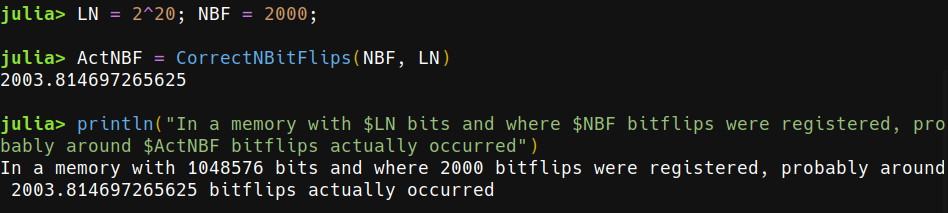
\includegraphics[width=0.75\columnwidth]{fig/functions/CorrectNBitFlips.png}
		\caption{Example of use of \texttt{CorrectNBitFlips}.}
		\label{fig:Example_CorrectNBitflips}
	\end{figure}
	
	Expression is taken from Eq. 6 in F. J. Franco, J. A. Clemente, H. Mecha and R. Velazco, 
	"\textit{Influence of Randomness During the Interpretation of Results From Single-Event Experiments 
		on SRAMs}," IEEE Transactions on Device and Materials Reliability, vol. 19, no. 1, pp. 104-111, 
	March 2019, doi: 10.1109/TDMR.2018.
	2886358.		
\end{itemize}
%
\subsubsection*{NF2BitMCUs}\label{Fun:NF2BitMCUs}
%
\begin{itemize}
	\item \textbf{Input arguments}: 
	\begin{itemize}
		\item \textit{Method 1}: \textbf{NSBU}::Int, \textbf{LA}::Int, \textbf{METHOD}::String, \textbf{D}::Int, \textbf{WordWidth}::Int, \textbf{UsePseudoAddress}::Bool
		\item \textit{Method 2}: \textbf{NSBU}::Int, \textbf{LA}::Int, \textbf{METHOD}::String, \textbf{D}::Int, \textbf{WordWidth}::Int
	\end{itemize}
	\item \textbf{Output}: Float64
	\item It indicates the expected number of false 2-bit MCUs that will occur 
	in a memory with \textbf{LA} words with \textbf{WORDWIDTH} bits each in which \textbf{NSBU} SBUs have occurred. In this analysis, 
	MCUS are sought using some grouping method (\textbf{METHOD}) with a generalized distance \textbf{D}.
	
	If \textbf{UsePseudoAddress} is not provided, its default value is \texttt{false}.
	
	Unlike \hyperref[Fun:NF3BitMCUs]{\texttt{NF3BitMCUs}}, two values are provided as outputs, called  ``\textit{optimistic}'' and ``\textit{pessimistic}''. The actual number of expected false events is somewhere between both values. So far, it is not possible to get  more accurate value, as explained in the theoretical development. Use the values as you may wish.
	
	Admitted values for \textbf{METHOD} and \textbf{D} are the following:
	
	\begin{enumerate}
		\item \textbf{METHOD}: \texttt{"MBU"} \(\rightarrow\) Only MBUs are sought. In this case, \textbf{D} is the \textbf{WORDWiDTH}.
		\item \textbf{METHOD}: \texttt{"MHD"} \(\rightarrow\)  Only possible if the user has been able to place the flipped	cell in the XY plane. Two cells are related if \(\left|x_1-x_2\right|+ \left|y_1-y_2\right|) \le D\). This  is the \textit{``Manhattan distance''}.
		\item \textbf{METHOD}: \texttt{"IND"} \(\rightarrow\)  Only possible if the user has been able to place the flipped	cell in the XY plane. Two cells are related if \(\max(\left|x_1-x_2\right|, \left|y_1-y_2\right|) \le D\). In mathematics, this is the \textit{"infinite distance"}.
		\item \textbf{METHOD}: \texttt{"THD"} \(\rightarrow\)  Only valid if pairs of bitflips are located in a linear bitstream and if the
		distance between cells is smaller than \textbf{D}: \(\left|x_1-x_2\right| \le D\).
		\item \textbf{METHOD}: \texttt{"XOR"}\(\rightarrow\)  Related pairs are got by means of statistical deviations. Addresses are XORed 
		and only if the value is one of the \textbf{D} possible critical values. If the WORD Addresses  
		is used instead of PSEUDOADDRESS, the memory size must be expressed in WORDs, \textbf{LA = LN/WordWidth}.
		IF SO, THE WORDWIDTH MUST BE PROVIDED.
		\item \textbf{METHOD}: \texttt{"POS"}\(\rightarrow\)  Identical to the previous one but with positive subtraction instead of XOR.
	\end{enumerate}
	
	For LELAPE, only the two last methods are of interest. However, the other methods are included in the tool in case you have used another strategy to combine bitflips and wish to know the background noise. Fig. \ref{fig:Example_NF2BitMCUs} is an example of use.
	
	\begin{figure}[h!]
		\centering
		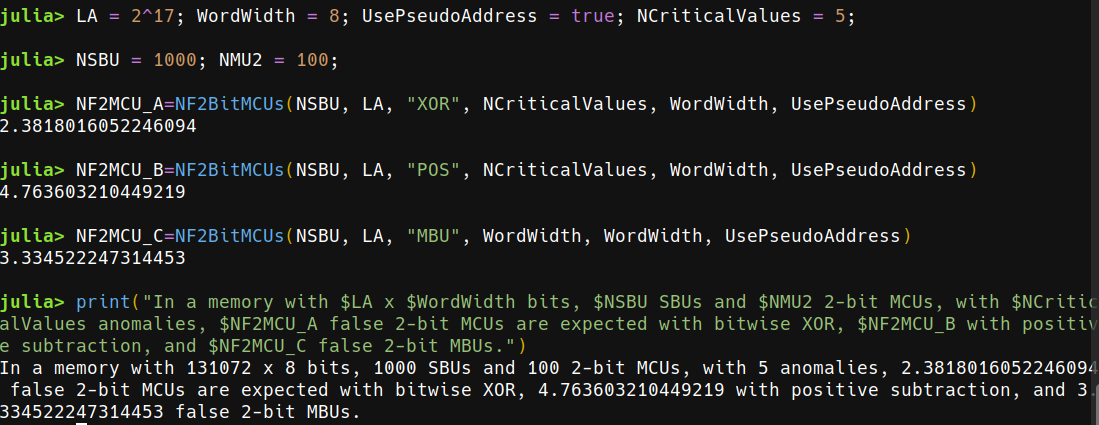
\includegraphics[width=0.75\columnwidth]{fig/functions/NF2BitMCUs.png}
		\caption{Example of use of \texttt{NF2BitMCUs}.}
		\label{fig:Example_NF2BitMCUs}
	\end{figure}	
	
	Everything can be found in Eq. 11 of F. J. Franco, J. A. Clemente, G. Korkian, 
	J. C. Fabero, H. Mecha and R. Velazco, "\textit{Inherent Uncertainty in the Determination of Multiple 
		Event Cross Sections in Radiation Tests,}" IEEE Transactions on Nuclear Science, vol. 67, no. 7, 
	pp. 1547-1554, July 2020, doi: 10.1109/TNS.2020.2977698.
	
\end{itemize}
%
\subsubsection*{NF3BitMCUs}\label{Fun:NF3BitMCUs}
%
\begin{itemize}
	\item \textbf{Input arguments}: 
	\begin{itemize}
		\item \textit{Method 1}: \textbf{NSBU}::Int, \textbf{NMU2}::Int, \textbf{LN}::Int, \textbf{METHOD}::String, \textbf{D}::Int, WordWidth::Int
		\item \textit{Method 2}: \textbf{NSBU}::Int, \textbf{NMU2}::Int, \textbf{LN}::Int, \textbf{METHOD}::String, \textbf{D}::Int
	\end{itemize}
	\item \textbf{Output}: Tuple{Float64, Float64}
	\item     It indicates the expected number of false 3-bit MCUs that will occur 	in a memory with \textbf{LN} bits in which \textbf{NSBU} SBUs and \textbf{NMU2} 2-bit MCUs have occurred. 	In this analysis, MCUS are sought using some grouping method (\textbf{METHOD}) with a generalized 
	distance D.
	
	MCUS are sought using some grouping method (\textbf{METHOD}) with a generalized distance \textbf{D}.
	
	Admitted values for \textbf{METHOD} and \textbf{D} are the following:
	
	\begin{enumerate}
	\item \textbf{METHOD}: \texttt{"MBU"} \(\rightarrow\) Only MBUs are sought. In this case, \textbf{D} is the \textbf{WORDWiDTH}.
	\item \textbf{METHOD}: \texttt{"MHD"} \(\rightarrow\)  Only possible if the user has been able to place the flipped	cell in the XY plane. Two cells are related if \(\left|x_1-x_2\right|+ \left|y_1-y_2\right|) \le D\). This  is the \textit{``Manhattan distance''}.
	\item \textbf{METHOD}: \texttt{"IND"} \(\rightarrow\)  Only possible if the user has been able to place the flipped	cell in the XY plane. Two cells are related if \(\max(\left|x_1-x_2\right|, \left|y_1-y_2\right|) \le D\). In mathematics, this is the \textit{"infinite distance"}.
	\item \textbf{METHOD}: \texttt{"THD"} \(\rightarrow\)  Only valid if pairs of bitflips are located in a linear bitstream and if the
	distance between cells is smaller than \textbf{D}: \(\left|x_1-x_2\right| \le D\).
	\item \textbf{METHOD}: \texttt{"XOR"}\(\rightarrow\)  Related pairs are got by means of statistical deviations. Addresses are XORed 
	and only if the value is one of the \textbf{D} possible critical values. If the WORD Addresses  
	is used instead of PSEUDOADDRESS, the memory size must be expressed in WORDs, \textbf{LA = LN/WordWidth}.
	IF SO, THE WORDWIDTH MUST BE PROVIDED.
	\item \textbf{METHOD}: \texttt{"POs"}\(\rightarrow\)  Identical to the previous one but with positive subtraction instead of XOR.
\end{enumerate}
	
	For LELAPE, only the two last methods are of interest. See Fig. \ref{fig:Example_NF3BitMCUs} for a practical example. However, the other methods are included in the tool in case you have used another strategy to combine bitflips and wish to know the background noise.
	
	\begin{figure}[h!]
		\centering
		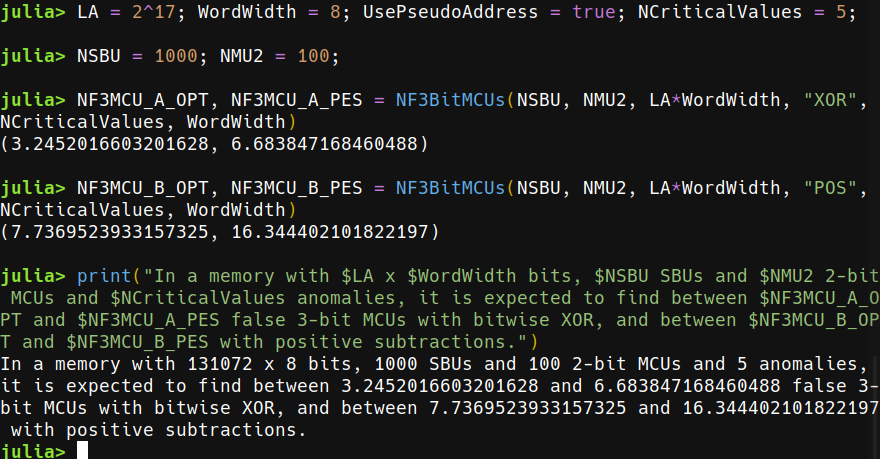
\includegraphics[width=0.75\columnwidth]{fig/functions/NF3BitMCUs.png}
		\caption{Example of use of \texttt{NF3BitMCUs}.}
		\label{fig:Example_NF3BitMCUs}
	\end{figure}	
	
	
	Everything can be found in Eq. 11 of F. J. Franco, J. A. Clemente, G. Korkian, 
	J. C. Fabero, H. Mecha and R. Velazco, "\textit{Inherent Uncertainty in the Determination of Multiple 
		Event Cross Sections in Radiation Tests,}" IEEE Transactions on Nuclear Science, vol. 67, no. 7, 
	pp. 1547-1554, July 2020, doi: 10.1109/TNS.2020.2977698.
	
	In this paper, it was demonstrated that it is mathematically impossible to get an exact value. Therefore,  optimistic and pessimistic results are provided.
\end{itemize}

\backmatter
\bibliographystyle{ieeetr}
\bibliography{LELAPE_bibliography.bib}

\end{document}